% !TeX spellcheck = <engl>

\let\textcircled=\pgftextcircled

\chapter{Results and Analysis}
\label{chap:results}

Following the described methodology in the previous chapter, this chapter seeks to interpret and analyse the results obtained while evaluating 


\section{Can We Automatically Detect Scene Contexts?}
\subsection{Metrics}
In evaluating the classifiers, it was  crucial to understand the predictive power of the two context classifiers. As such, precision, recall and f1-score were selected as the main performance metrics. 
\paragraph{Precision} is the percentage of positive predictions that were correct. 
\begin{equation*}
\centering
Precision=\frac{TP}{TP+FP}
\end{equation*}
\paragraph{Recall} is the percentage of positive samples that were correctly predicted. 
\begin{equation*}
\centering
Recall=\frac{TP}{TP+FN}
\end{equation*}
\paragraph{F1-score} is the balanced mean of the precision and recall.  
\begin{equation*}
\centering 
2\cdot\frac{precision\cdot recall}{precision+recall}
\end{equation*}
\subsection{Analysis}
Tables \ref{tab:penalisedpcl} and \ref{tab:context} form the basis of this analysis.

I established that determining the context from images is much more accurate than from point clouds. As highlighted before, images offer higher representational power and resolution than sparse point clouds. As seen in figure 41, the f1-score of the image classifier outperformed the point cloud classifier by more than 30\% . 


\begin{table}[h] % Context detection
	\centering
	\resizebox{\textwidth}{!}{%
		\begin{tabular}{|
				>{\columncolor[HTML]{FFFFFF}}l |
				>{\columncolor[HTML]{FFFFC7}}l |
				>{\columncolor[HTML]{FFFFC7}}l |
				>{\columncolor[HTML]{FFFFC7}}l |
				>{\columncolor[HTML]{FFFFC7}}l |
				>{\columncolor[HTML]{96FFFB}}l |
				>{\columncolor[HTML]{96FFFB}}l |
				>{\columncolor[HTML]{96FFFB}}l |
				>{\columncolor[HTML]{96FFFB}}l |}
			\hline
			{\color[HTML]{333333} \textbf{}} & \multicolumn{4}{l|}{\cellcolor[HTML]{FFFFC7}{\color[HTML]{333333} \textbf{Context Detection using PointCloud Feature Matching}}} & \multicolumn{4}{l|}{\cellcolor[HTML]{96FFFB}\textbf{Context Detection using Image Segmentation}} \\ \hline
			{\color[HTML]{333333} \textbf{Context}} & {\color[HTML]{333333} \textbf{precision}} & {\color[HTML]{333333} \textbf{recall}} & {\color[HTML]{333333} \textbf{f1-score}} & {\color[HTML]{333333} \textbf{support}} & \textbf{precision} & \textbf{recall} & \textbf{f1-score} & \textbf{support} \\ \hline
			{\color[HTML]{333333} \textit{\textbf{urban}}} & {\color[HTML]{333333} \textbf{0.52}} & {\color[HTML]{333333} 0.45} & {\color[HTML]{333333} 0.48} & {\color[HTML]{333333} 206} & 0.81 & \textbf{0.9} & \textbf{0.85} & 193 \\ \hline
			{\color[HTML]{333333} \textit{\textbf{non-urban}}} & {\color[HTML]{333333} 0.51} & {\color[HTML]{333333} \textbf{0.58}} & {\color[HTML]{333333} \textbf{0.55}} & {\color[HTML]{333333} 206} & \textbf{0.9} & 0.81 & \textbf{0.85} & 218 \\ \hline
			{\color[HTML]{333333} \textbf{avg / total}} & {\color[HTML]{333333} 0.51} & {\color[HTML]{333333} 0.51} & {\color[HTML]{333333} 0.51} & {\color[HTML]{333333} 412} & 0.86 & 0.85 & 0.85 & 411 \\ \hline
		\end{tabular}%
	}
	\caption{Comparison of context detection methods}
	\label{tab:context}
\end{table}

With regard to the point cloud context classifier, majority voting resulted in around 50:50 precision for both classes. The recall for the non-urban was 7 percent more than urban which was below 50\%. By implementing the penalty function in the point cloud classifier, recall for the urban class improved by 17\%  as seen in table \ref{tab:penalisedpcl}. 

\begin{table}[h] % Penalised
	\centering
	\begin{tabular}{|l|l|l|l|l|}
		\hline
		\multicolumn{5}{|l|}{\textbf{Penalised Point Cloud Context Classifier}}                            \\ \hline
		\textbf{context}            & \textbf{precision} & \textbf{recall} & \textbf{f1-score} & \textbf{support} \\ \hline
		\textbf{urban}       & \textbf{0.52}      & \textbf{0.62}   & \textbf{0.54}     & 206              \\ \hline
		\textbf{non-urban}   & 0.46               & 0.33            & 0.38              & 206              \\ \hline
		\textbf{avg / total} & 0.47               & 0.47            & 0.46              & 412              \\ \hline
	\end{tabular}
	\caption{Penalised Point Cloud classifier}
	\label{tab:penalisedpcl}
\end{table}

\section{Do Object Detection Models Perform Better in Different Contexts?}
\subsection*{Metrics}
\subsubsection*{KITTI Evaluation Protocol}
The models were evaluated using the official KITTI evaluation protocol. Average precision(AP) is the area under a recall-precision curve that was calculated after predictions. Predicted bounding boxes were considered as positive matched if they were above a predefined intersection over union(IoU). 
IoU is calculated as: \\ 
\begin{math}
\centering
IoU = \frac{Overlap\, area}{Union\, area}
\end{math} \\ 
Where the overlap area is the region that is shared between the predicted bounding box and the ground truth bounding box and the Union area is the total area of the predicted bounding box and ground truth box.
This was calculated for 2D bounding boxes, 3D bounding boxes and Bird-Eye View bounding boxes. The IoU threshold was set at  $\geq$0.7 for the car class and $\geq$0.5 for the pedestrian class. 

\subsubsection*{GPU}
As mentioned earlier, the resources of an AV are limited and therefore it is encouraged to implement efficient models. In light of this, I monitored the GPU statistics to better understand how different models affect the GPU. 
During inference, GPU statistics were collected at an interval of 1 second using NVIDIA System Management Interface(nvidia-smi). The following metrics were collected. 
\begin{itemize}[noitemsep]
	\item \textbf{Power Draw } - Watts
	\item \textbf{Memory Used } - MB
	\item \textbf{Temperature} - $\degree$C
	\item \textbf{Clock Speed} - MHz
\end{itemize}
For uniformity purposes, all the experiments were performed on single NVIDIA P100 GPU with 16GB High Bandwidth Memory. 
\subsubsection*{Baseline}
 A baseline, was established by running each model was run on the original KITTI validation dataset. The results can be seen in table  in \ref{tab:baseline}. In addition, the temperature and power metrics were collected and can be seen in the last boxplot of figures \ref{fig:temp} and \ref{fig:power}.

\begin{table}[H] %baseline
	\centering
	\resizebox{\textwidth}{!}{%
		\begin{tabular}{|l|l|
				>{\columncolor[HTML]{FFCCC9}}l |
				>{\columncolor[HTML]{FFCCC9}}l |
				>{\columncolor[HTML]{FFCCC9}}l |
				>{\columncolor[HTML]{96FFFB}}l |
				>{\columncolor[HTML]{96FFFB}}l |
				>{\columncolor[HTML]{96FFFB}}l |}
			\hline
			& \textbf{Class}                     & \multicolumn{3}{l|}{\cellcolor[HTML]{FFCCC9}{\color[HTML]{000000} \textbf{Car}}}                                                  & \multicolumn{3}{l|}{\cellcolor[HTML]{96FFFB}{\color[HTML]{000000} \textbf{Pedestrian}}}                                           \\ \hline
			\textbf{Model}               & \textbf{Difficulty}                & {\color[HTML]{000000} \textbf{Easy}}      & {\color[HTML]{000000} \textbf{Medium}}    & {\color[HTML]{000000} \textbf{Hard}}      & {\color[HTML]{000000} \textbf{Easy}}      & {\color[HTML]{000000} \textbf{Medium}}    & {\color[HTML]{000000} \textbf{Hard}}      \\ \hline
			& \textit{\textbf{2D Bounding Box}}  & {\color[HTML]{000000} \textbf{86.987999}} & {\color[HTML]{000000} \textbf{77.10569}}  & {\color[HTML]{000000} \textbf{68.012459}} & {\color[HTML]{000000} 56.214417}          & {\color[HTML]{000000} 51.969517}          & {\color[HTML]{000000} 46.578247}          \\ \cline{2-8} 
			& \textit{\textbf{BEV Bounding Box}} & {\color[HTML]{000000} \textbf{86.00412}}  & {\color[HTML]{000000} \textbf{74.355942}} & {\color[HTML]{000000} \textbf{65.62397}}  & {\color[HTML]{000000} \textbf{50.94368}}  & {\color[HTML]{000000} \textbf{49.857227}} & {\color[HTML]{000000} \textbf{44.704525}} \\ \cline{2-8} 
			\multirow{-3}{*}{\textbf{AVOD}}     & \textit{\textbf{3D Bounding Box}}  & {\color[HTML]{000000} \textbf{75.447769}} & {\color[HTML]{000000} \textbf{63.742085}} & {\color[HTML]{000000} \textbf{54.334251}} & {\color[HTML]{000000} \textbf{48.757492}} & {\color[HTML]{000000} \textbf{44.84359}}  & {\color[HTML]{000000} \textbf{43.014023}} \\ \hline
			& \textit{\textbf{2D Bounding Box}}  & {\color[HTML]{000000} 65.951279}          & {\color[HTML]{000000} 56.683437}          & {\color[HTML]{000000} 55.972511}          & {\color[HTML]{000000} \textbf{66.309807}} & {\color[HTML]{000000} \textbf{60.556213}} & {\color[HTML]{000000} \textbf{53.479141}} \\ \cline{2-8} 
			& \textit{\textbf{BEV Bounding Box}} & {\color[HTML]{000000} 81.242409}          & {\color[HTML]{000000} 70.672707}          & {\color[HTML]{000000} 65.347595}          & {\color[HTML]{000000} 50.308723}          & {\color[HTML]{000000} 46.726196}          & {\color[HTML]{000000} 41.24551}           \\ \cline{2-8} 
			\multirow{-3}{*}{\textbf{VoxelNet}} & \textit{\textbf{3D Bounding Box}}  & {\color[HTML]{000000} 40.000149}          & {\color[HTML]{000000} 34.892159}          & {\color[HTML]{000000} 31.376112}          & {\color[HTML]{000000} 34.161884}          & {\color[HTML]{000000} 30.576441}          & {\color[HTML]{000000} 28.982103}          \\ \hline
		\end{tabular}%
	}
	\caption{Baseline}
	\label{tab:baseline}
\end{table}

\subsubsection{Running Each Model Exclusively}
To investigate whether the performance of each model varies in different contexts, each model was run exclusively on a single GPU with data from each context dataset. 

\begin{table}[h] %Car AP
	\centering
	\resizebox{\textwidth}{!}{%
		\begin{tabular}{|l|l|
				>{\columncolor[HTML]{FFCCC9}}l |
				>{\columncolor[HTML]{FFCCC9}}l |
				>{\columncolor[HTML]{FFCCC9}}l |
				>{\columncolor[HTML]{96FFFB}}l |
				>{\columncolor[HTML]{96FFFB}}l |
				>{\columncolor[HTML]{96FFFB}}l |}
			\hline
			\textbf{}                           & \textbf{Context}                   & \multicolumn{3}{l|}{\cellcolor[HTML]{FFCCC9}\textbf{Urban}}  & \multicolumn{3}{l|}{\cellcolor[HTML]{96FFFB}\textbf{Non-Urban}} \\ \hline
			\textbf{Model}                           & \textbf{Difficulty}                & \textbf{Easy}      & \textbf{Medium}    & \textbf{Hard}      & \textbf{Easy}       & \textbf{Medium}     & \textbf{Hard}       \\ \hline
			\multirow{3}{*}{\textbf{AVOD}} & \textit{\textbf{2D Bounding Box}} & \textbf{86.987999} & \textbf{77.10569} & \textbf{68.012459} & \textbf{89.186172} & \textbf{79.754562} & \textbf{78.550514} \\ \cline{2-8} 
			& \textit{\textbf{BEV Bounding Box}} & 86.00412 & 74.355942 & 65.62397 & 87.11274 & \textbf{76.859818} & \textbf{75.720955} \\ \cline{2-8} 
			& \textit{\textbf{3D Bounding Box}} & \textbf{75.447769} & \textbf{63.742085} & \textbf{54.334251} & \textbf{75.430656} & \textbf{64.199951} & \textbf{62.902302} \\ \hline
			\multicolumn{1}{|c|}{\multirow{3}{*}{\textbf{VoxelNet}}} & \textit{\textbf{2D Bounding Box}} & 69.597939 & 65.98201 & 59.284454 & 77.520409 & 67.733231 & 62.281651 \\ \cline{2-8} 
			\multicolumn{1}{|c|}{} & \textit{\textbf{BEV Bounding Box}} & \textbf{86.34037} & \textbf{76.187859} & \textbf{68.103294} & \textbf{88.635025} & 75.361214 & 69.502548 \\ \cline{2-8} 
			\multicolumn{1}{|c|}{} & \textit{\textbf{3D Bounding Box}} & 73.632263 & 58.473991 & 50.744587 & 68.620865 & 49.455608 & 45.809917 \\ \hline
		\end{tabular}%
	}
	\caption{Car AP}
	\label{tab:cardetap}
\end{table}
\begin{table}[h]%Pedestrian AP
	\centering
	\resizebox{\textwidth}{!}{%
		\begin{tabular}{|l|l|
				>{\columncolor[HTML]{FFCCC9}}l |
				>{\columncolor[HTML]{FFCCC9}}l |
				>{\columncolor[HTML]{FFCCC9}}l |
				>{\columncolor[HTML]{96FFFB}}l |
				>{\columncolor[HTML]{96FFFB}}l |
				>{\columncolor[HTML]{96FFFB}}l |}
			\hline
			\textbf{}                           & \textbf{Context}                   & \multicolumn{3}{l|}{\cellcolor[HTML]{FFCCC9}\textbf{Urban}}  & \multicolumn{3}{l|}{\cellcolor[HTML]{96FFFB}\textbf{Non-Urban}} \\ \hline
			\textbf{Model}                           & \textbf{Difficulty}                & \textbf{Easy}      & \textbf{Medium}    & \textbf{Hard}      & \textbf{Easy}       & \textbf{Medium}     & \textbf{Hard}       \\ \hline
			& \textit{\textbf{2D Bounding Box}}  & \textbf{78.626633} & \textbf{77.407684} & \textbf{70.029228} & 76.096977           & 70.946465           & 71.205276           \\ \cline{2-8} 
			& \textit{\textbf{BEV Bounding Box}} & \textbf{80.880447} & \textbf{80.393105} & \textbf{79.296593} & 77.806831           & 77.654358           & 71.792923           \\ \cline{2-8} 
			\multirow{-3}{*}{\textbf{AVOD}}     & \textit{\textbf{3D Bounding Box}}  & \textbf{80.649719} & \textbf{80.142876} & \textbf{79.056778} & 77.538368           & 71.868484           & 71.564285           \\ \hline
			& \textit{\textbf{2D Bounding Box}}  & 72.129387          & 65.245384          & 65.508232          & \textbf{84.218407}  & \textbf{76.52832}   & \textbf{76.593803}  \\ \cline{2-8} 
			& \textit{\textbf{BEV Bounding Box}} & 74.766678          & 73.944069          & 74.138588          & \textbf{89.830276}  & \textbf{80.201164}  & \textbf{80.114815}  \\ \cline{2-8} 
			\multirow{-3}{*}{\textbf{VoxelNet}} & \textit{\textbf{3D Bounding Box}}  & 71.177628          & 64.247559          & 64.18145           & \textbf{87.206612}  & \textbf{77.964493}  & \textbf{78.036652}  \\ \hline
		\end{tabular}%
	}
	\caption{Pedestrian AP}
	\label{tab:pedap}
\end{table}


\begin{figure}[H] %Power&Temp
	\centering
	\begin{minipage}[b]{\textwidth}
		\centering
		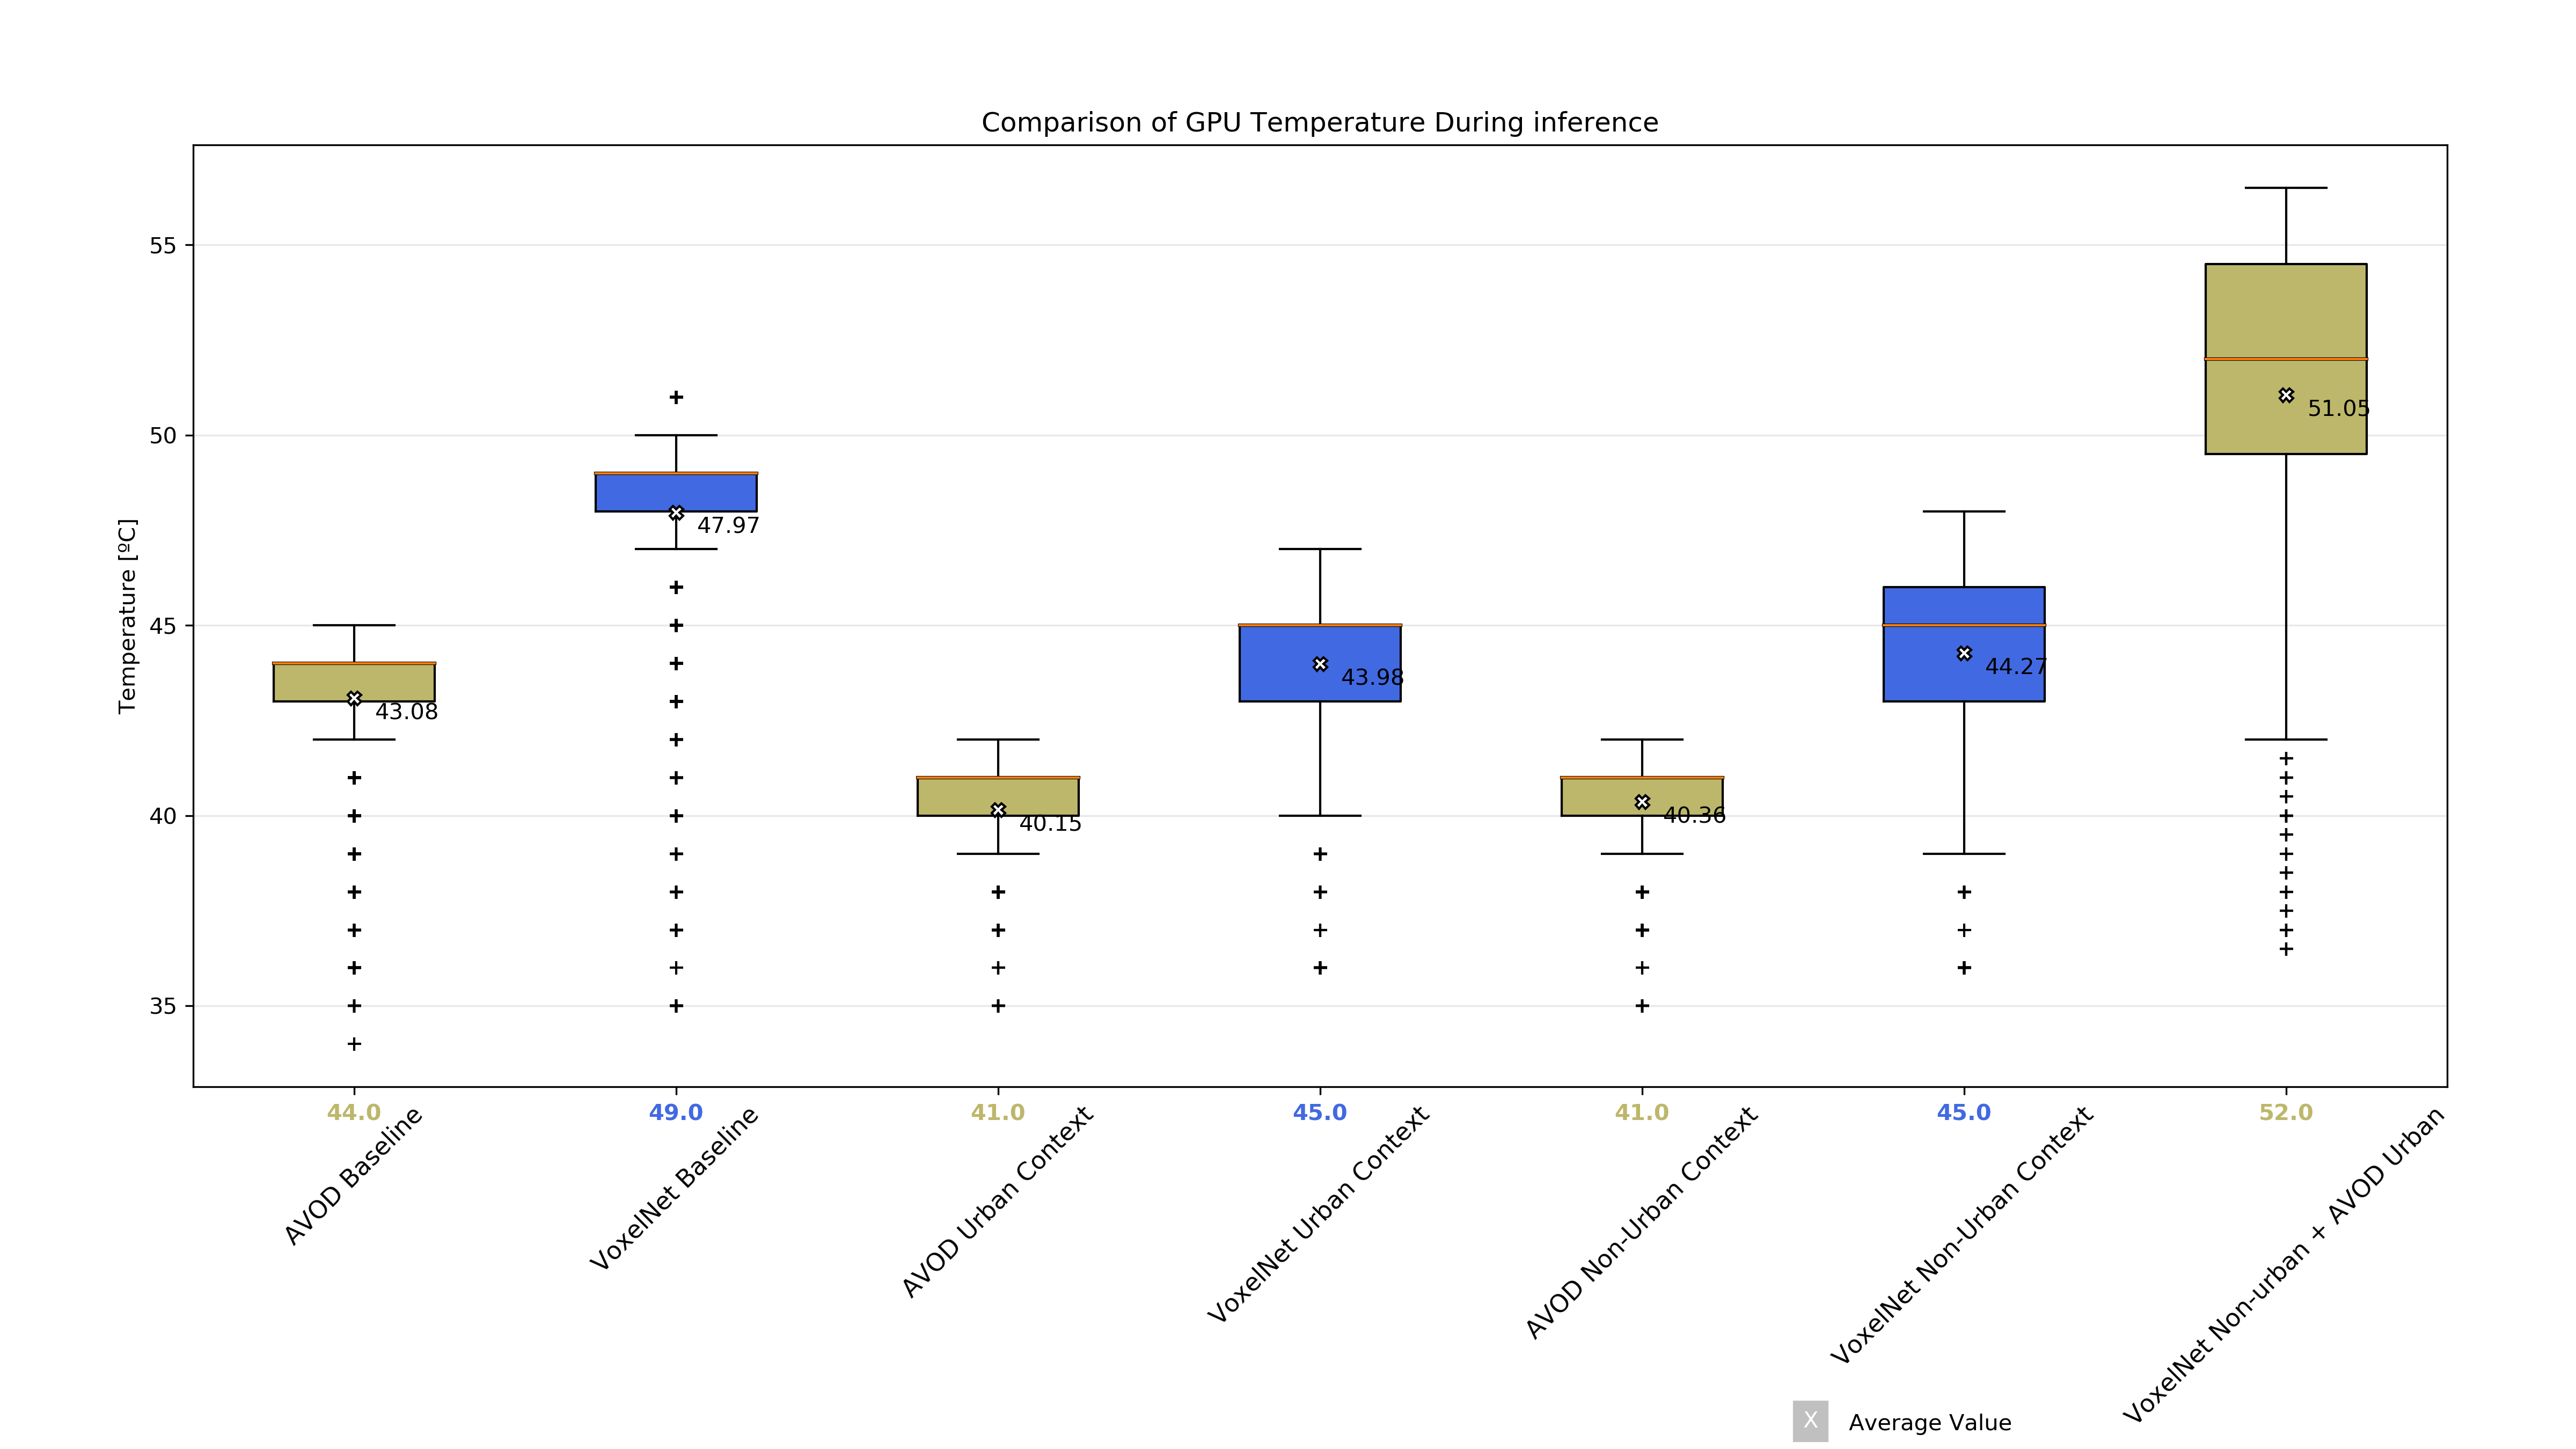
\includegraphics[width=\textwidth]{images/gputepbox.png}
		\caption{Temperature boxplots of evaluation runs.Voxelnet(blue) AVOD(gold) AVOD+VoxelNet(Red)}
		\label{fig:temp}
	\end{minipage}
	%	\hfill
	\begin{minipage}[b]{\textwidth}
		\centering
		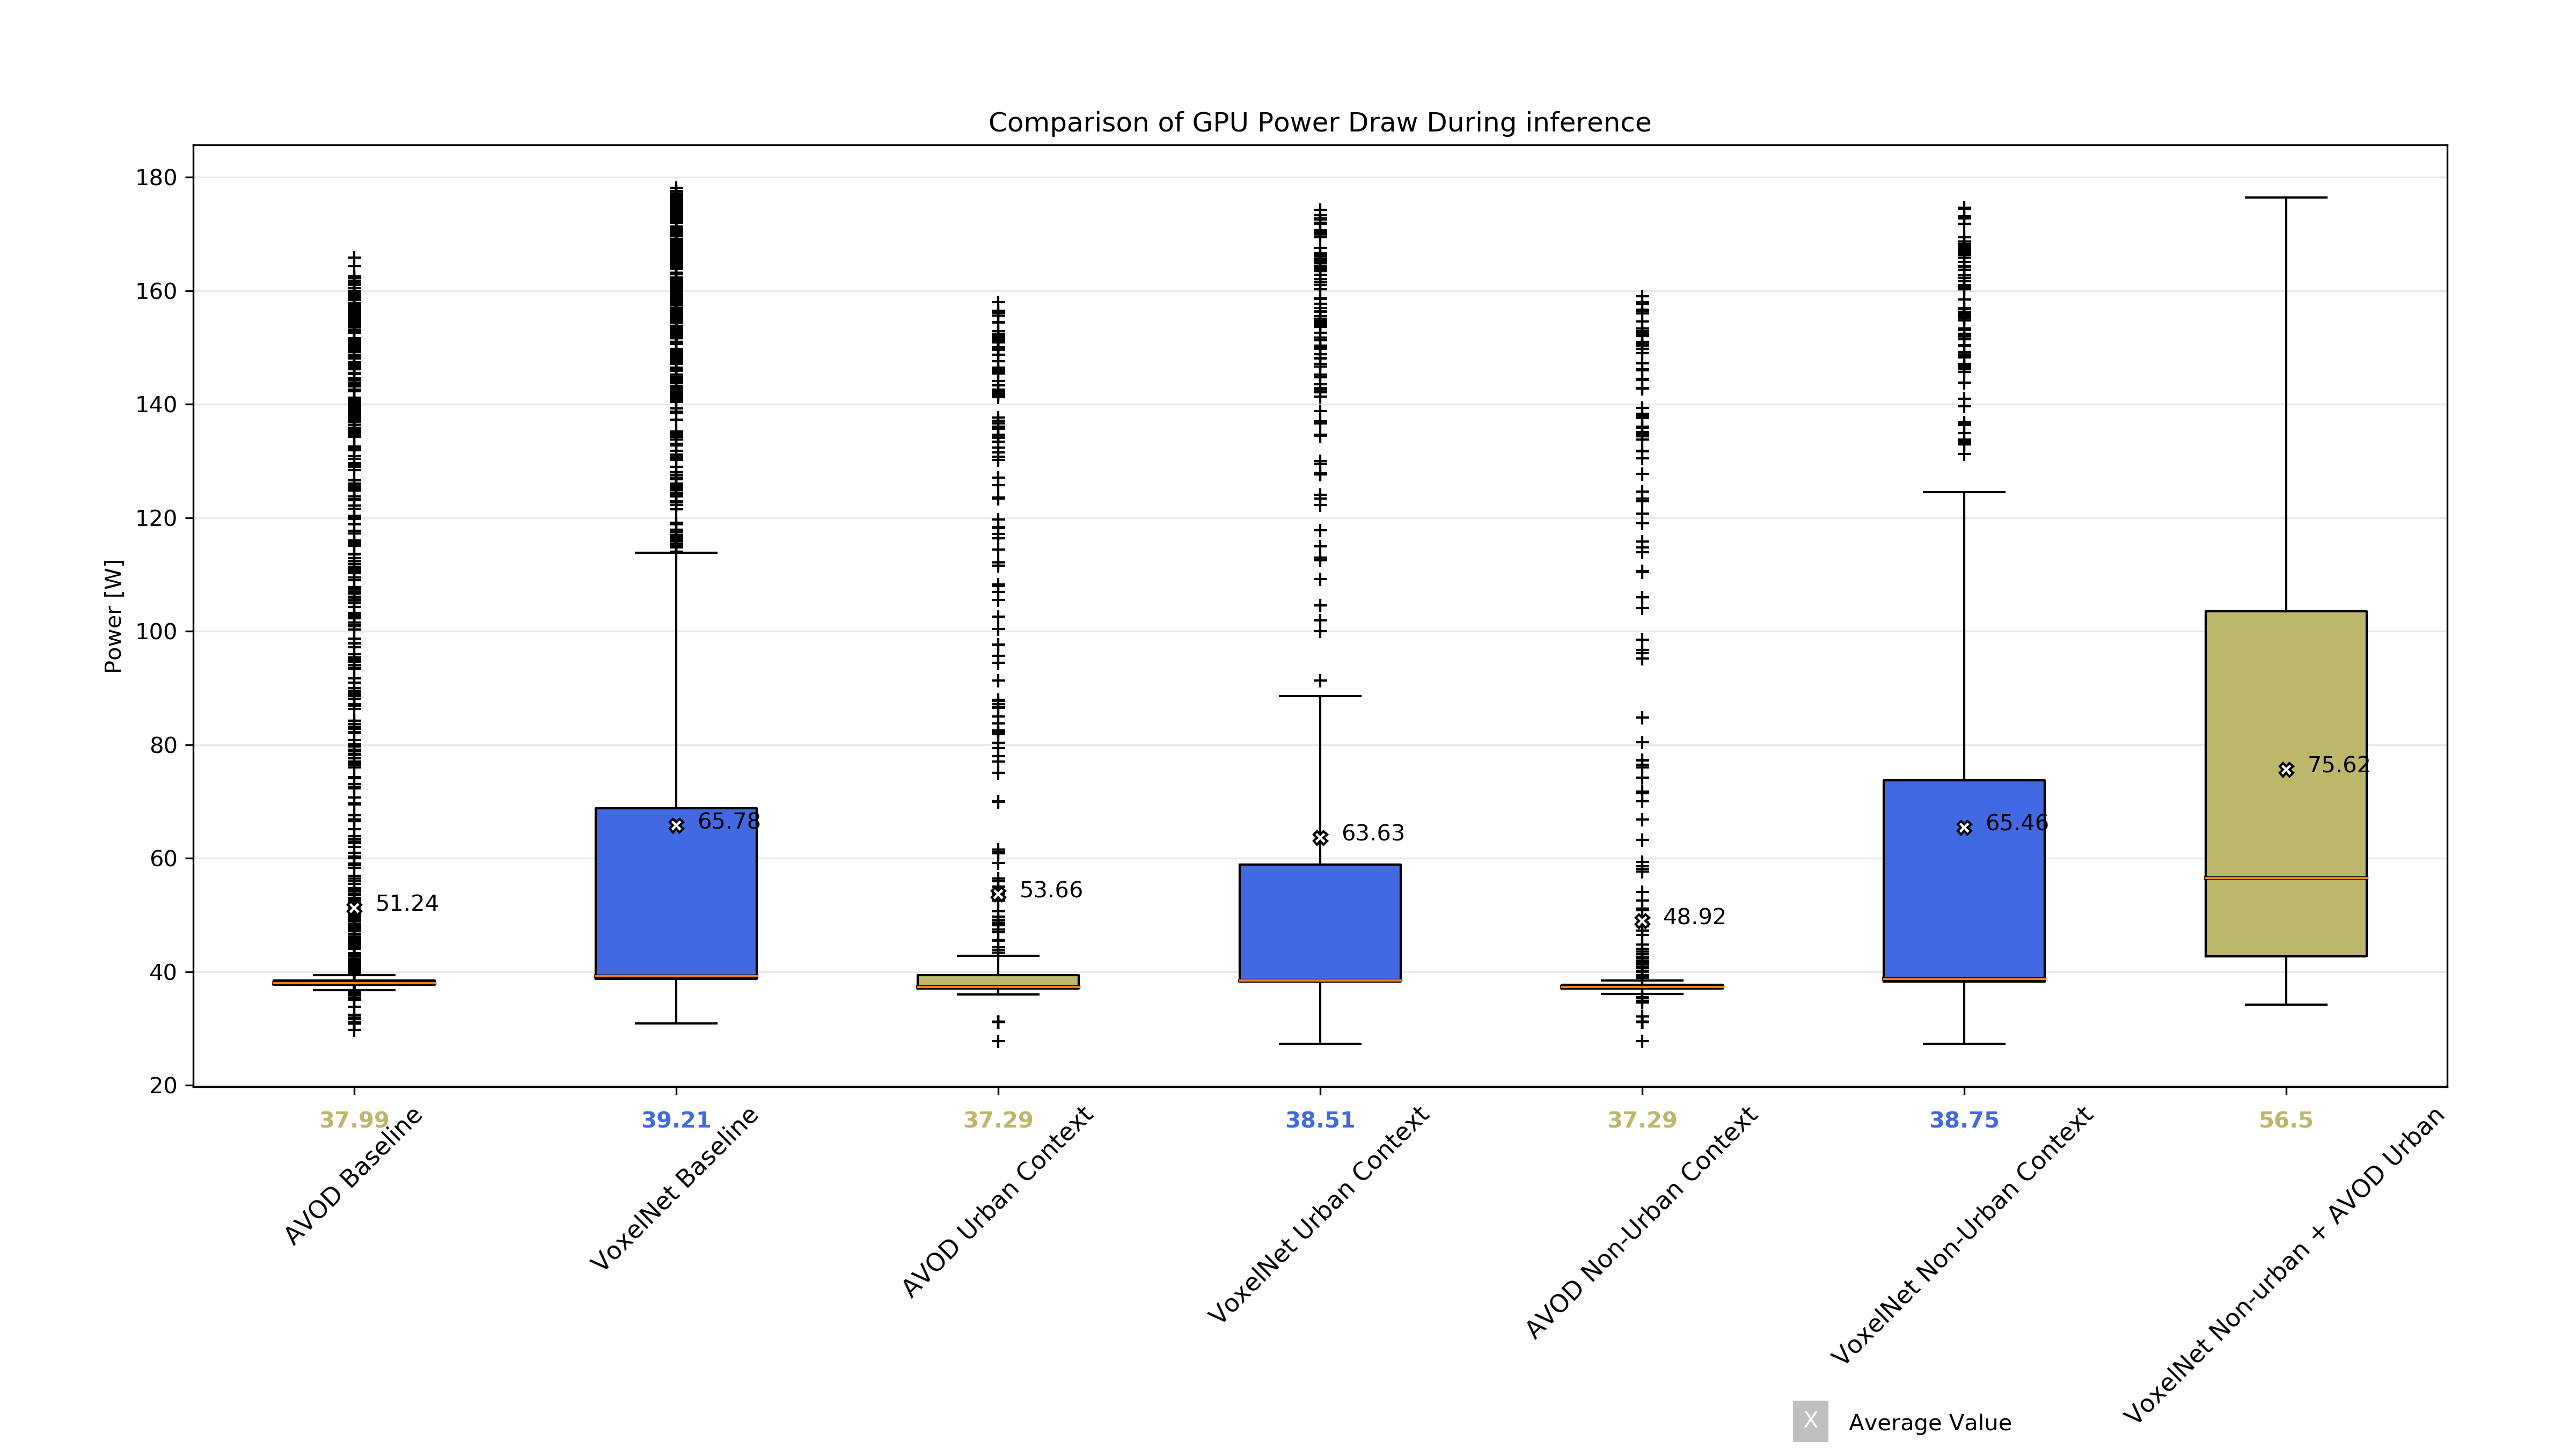
\includegraphics[width=\textwidth]{images/gpupbox.png}
		\caption{Power boxplots of evaluation runs. Voxelnet(blue), AVOD(gold), AVOD+VoxelNet(Red}
		\label{fig:power}
	\end{minipage}
	
\end{figure}


\subsubsection*{Analysis}
The qualitative results of the models are illustrated in tables \ref{tab:cardetap}, \ref{tab:pedap} and \ref{tab:inftime} .Results for the urban context are highlighted in pink whereas non-urban results are highlighted in blue. GPU results are available in form of boxplots on figures \ref{fig:power} and \ref{fig:temp}. For this evaluation, the first six boxplots form the basis of this analysis. The median is highlighted at the bottom of the x-axis in gold and blue while the average is in black font next to the 'X' marker.



\paragraph{Car} - AVOD outperformed VoxelNet on 2D and 3D detections in both contexts. However, VoxelNet performed slightly better in bird-eye-view detections as compared to AVOD. 
\paragraph{Pedestrian} - As compared to the car class, there was a distinct performance boundary whereby AVOD dominated all detections in the urban context whereas VoxelNet did in the non-urban context.

\begin{table}[h]%Time
	\centering
	%	\resizebox{\textwidth}{!}{%
	\begin{tabular}{|l|l|l|l|l|l|l|}
		\hline
		\multirow{2}{*}{\textbf{Context}} & \multicolumn{3}{l|}{\textbf{VoxelNet}} & \multicolumn{3}{c|}{\textbf{AVOD}} \\ \cline{2-7} 
		& \textbf{min} & \textbf{max} & \textbf{mean} & \textbf{min} & \textbf{max} & \textbf{mean} \\ \hline
		\textbf{Urban} & 0.113 & 3.813 & 0.129 & \textbf{0.095} & \textbf{2.457} & \textbf{0.112} \\ \hline
		\textbf{Non-urban} & 0.113 & \textbf{2.224} & 0.127 & \textbf{0.096} & 2.506 & \textbf{0.113} \\ \hline
	\end{tabular}%
	%	}
	\caption{Inference Time on Single NVIDIA P100 GPU}
	\label{tab:inftime}
\end{table}

In terms of inference time, AVOD was slightly faster than VoxelNet in both contexts Notably, the minimum time for VoxelNet was AVOD's mean time. Nonetheless both were able to achieve a frame rate of about \textbf{9 FPS}. 

\paragraph{GPU} - As seen in figures \ref{fig:power} and \ref{fig:temp},AVOD generally ran at a lower temperature and consumed less power as compared to VoxelNet. 
Generally, VoxelNet caused higher temperatures more than 75\% of the time. The spread of temperature was smaller for AVOD as compared to VoxelNet's. 
In terms of \textbf{power usage}, a similar pattern was seen whereby the AVOD's usage stabilised within a very small range most of the time as compared to VoxelNet which exhibited  a significantly higher range fluctuation. 
With regard to the context, running the models on a specific context resulted in lower median temperatures as seen in figure 41. For VoxelNet, the median temperature reduced by around 4\degree Celsius whereas for AVOD the median temperature was reduced by around 3\degree  Celsius. Additionally, VoxelNet had a smaller spread while running on the urban context as compared to VoxelNet. AVOD did not exhibit any significant changes in terms of spread while running in different contexts. AVOD's and VoxelNet's median power usage did not exhibit any significant reduction. However, AVOD running in a non-urban context resulted in a very small spread with a slightly lower mean temperature as compared to running in an urban context. An opposite effect was seen in VoxelNet's spread where running in a non-urban context resulted in a larger spread and slightly higher mean temperature.


\subsubsection*{Running Both Models Simultaneously}
Having identified that AVOD is better at detecting cars and pedestrians in urban contexts and VoxelNet in non-urban contexts, I set out to further investigate whether it is possible to have both models running optimally on a single GPU. This was done by running both models simultaneously. Each model was started on an initial memory fraction of 40\%(6.4GB) and was allowed to grow. This was done by setting the \textit{\textbf{gpu\_mem\_fraction}} to \textbf{0.4} and \textbf{\textit{allow\_mem\_growth}} to \textbf{True} before running the respective Tensorflow graphs. 

\begin{table}[H] % memory
	\centering
	\caption{Memory}
	\label{tab:mem}
	\begin{tabular}{|l|l|l|}
		\hline
		& \textbf{Min} & \textbf{Max} \\ \hline
		\textbf{Memory(MB)} & 4608.50  & 14320.00\\ \hline
	\end{tabular}
	
\end{table}

\subsubsection*{Analysis}
The results are available in form of boxplots on figures \ref{fig:power} and \ref{fig:temp} as well as table \ref{tab:mem}. For this test, the last boxplot forms the basis of this analysis.The median is highlighted at the bottom of the x-axis in red while the average is in black font next to the 'X' marker.
\paragraph{Temperature} - Running both models simultaneously resulted in significantly higher temperatures as compared running them exclusively. The average temperature was 7\degree hotter than the maximum mean temperature from running the models exclusively. In addition, the temperature exhibited a significantly greater spread than running either model on any context.
\paragraph{Power} - A similar trend was seen power-wise. The mean power usage was 10 watts greater than the maximum mean power from running the models exclusively. In addition, the spread of power was much larger than running either context. The median power usage was also much higher by around 16 Watts. 
\paragraph{Memory} - Running both models resulted in a total memory usage of 14.3 GB out of the total memory of 16GB. Both models were able to run optimally with no memory exhaustion errors. 

\section{Is VoxelNet Performance Valid For Different Datasets?}
\subsection*{Metrics}
Given that the data was collected from a stationary vehicle in an urban area with mostly pedestrians,  VoxelNet was evaluated on the pedestrian class only. However, as there was no corresponding image data for the point clouds, only the 3D bounding boxes and Bird-Eye View bounding boxes with IoU $\geq$ 0.5. were used in calculating the AP. 
\subsection*{Analysis}
VoxelNet was \textbf{not} able to predict any objects on the SIL dataset. As highlighted before, the VLP-16 LiDAR sensor has a lower frequency than that of the HDL-64E. This therefore affected the point cloud density and is visible in figure \ref{fig:difference}. From this figure, we can see that more SIL point cloud density was significantly lower than that of KITTI. SIL point clouds had an average point cloud density per frame that was lower than that of KITTI's by 42\%  with a median of 0.0048 in 1000 samples as seen in figure \ref{fig:density} as compared to SIL's of 0.0028. In fact, close to 100\% of the KITTI point cloud density was higher than that of SIL. Nonetheless, the KITTI point cloud density fluctuated along a larger range as compared to the SIL dataset.

The point cloud density was calculated as: 

$density = \frac{N_{i}}{S_{i}}  $  \\
where N is the number of points in point cloud frame \textit{i} and S is the XY size of the frame \textit{i}.

\begin{figure}[H] %SIL KITTI
	\centering
	\begin{minipage}[b]{0.49\textwidth}
		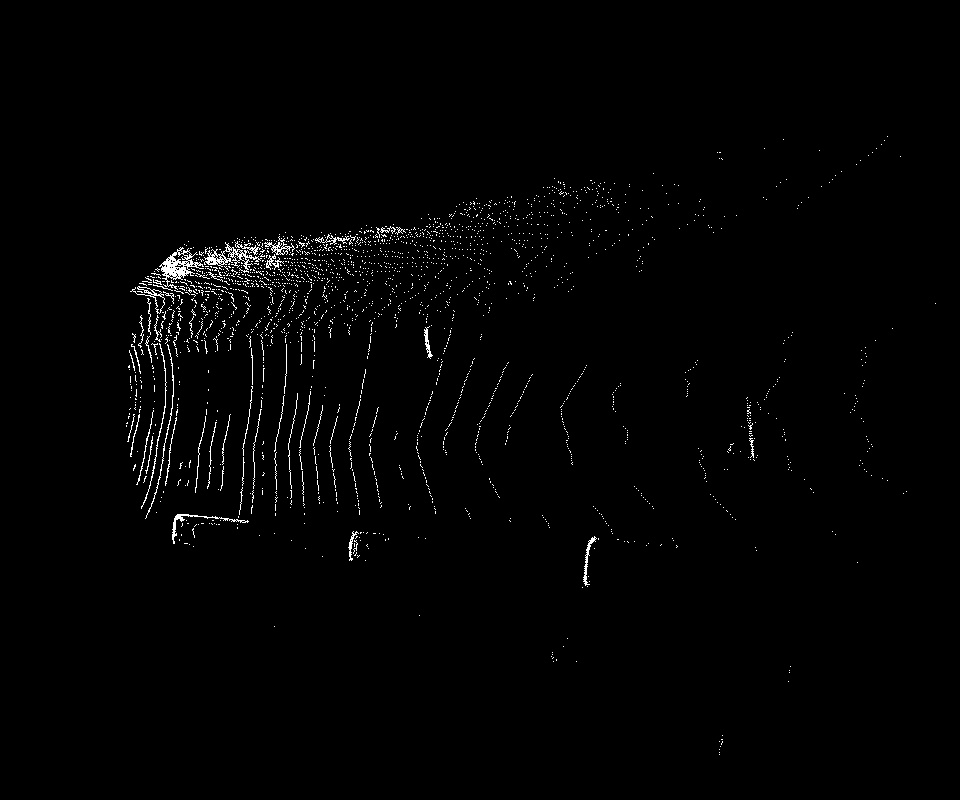
\includegraphics[width=\textwidth,height=6.5cm]{images/kitti_bv}
		\caption*{KITTI bird eye view}
%	\label{fig:kittibv}
	\end{minipage}
	%	\hfill
	\begin{minipage}[b]{0.49\textwidth}
		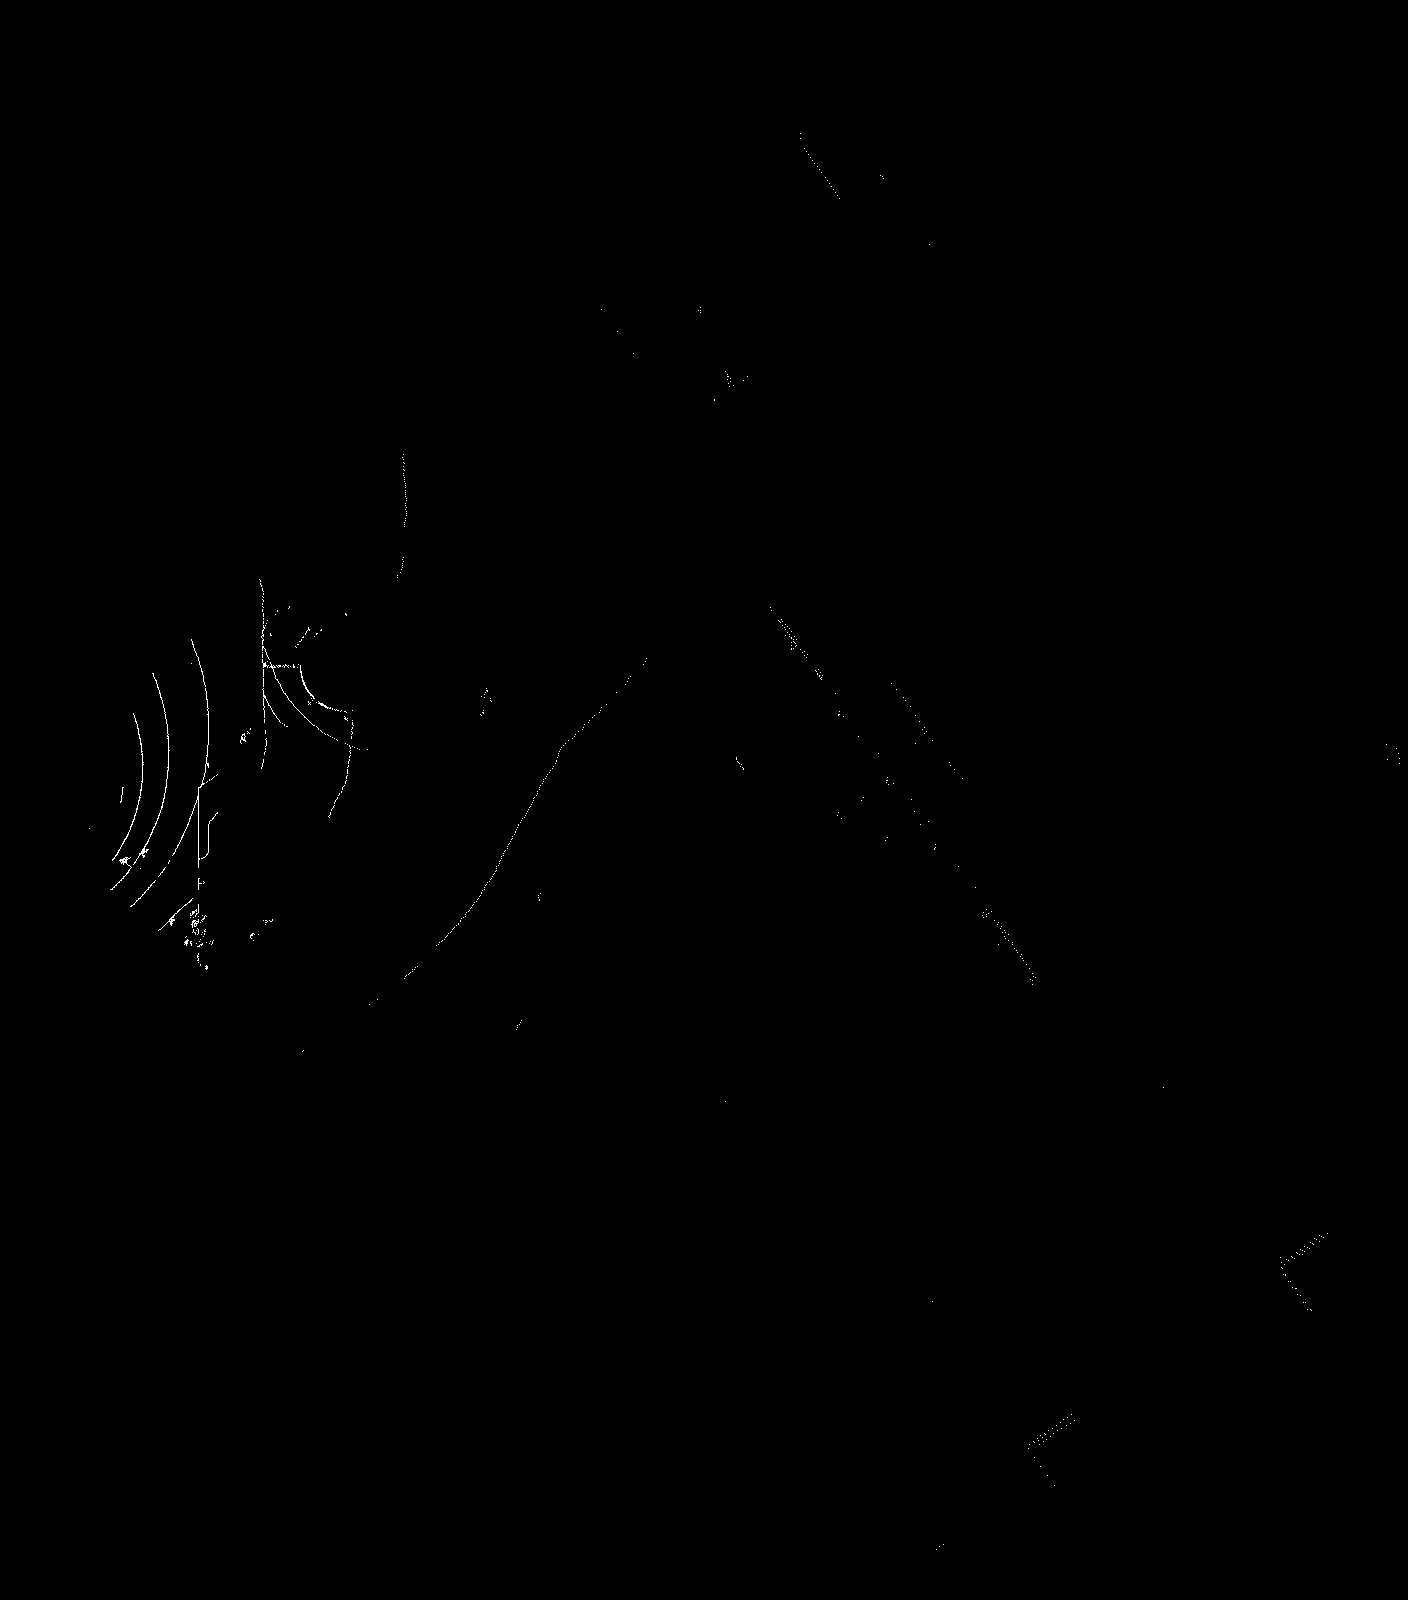
\includegraphics[width=\textwidth,height=6.5cm]{images/sil_bv}
		\caption*{SIL bird eye view}
%		\label{fig:silbv}
	\end{minipage}
	\caption{Bird Eye View Difference between SIL and KITTI}
	\label{fig:difference}
\end{figure}

\begin{figure}[H] % density
	\centering
	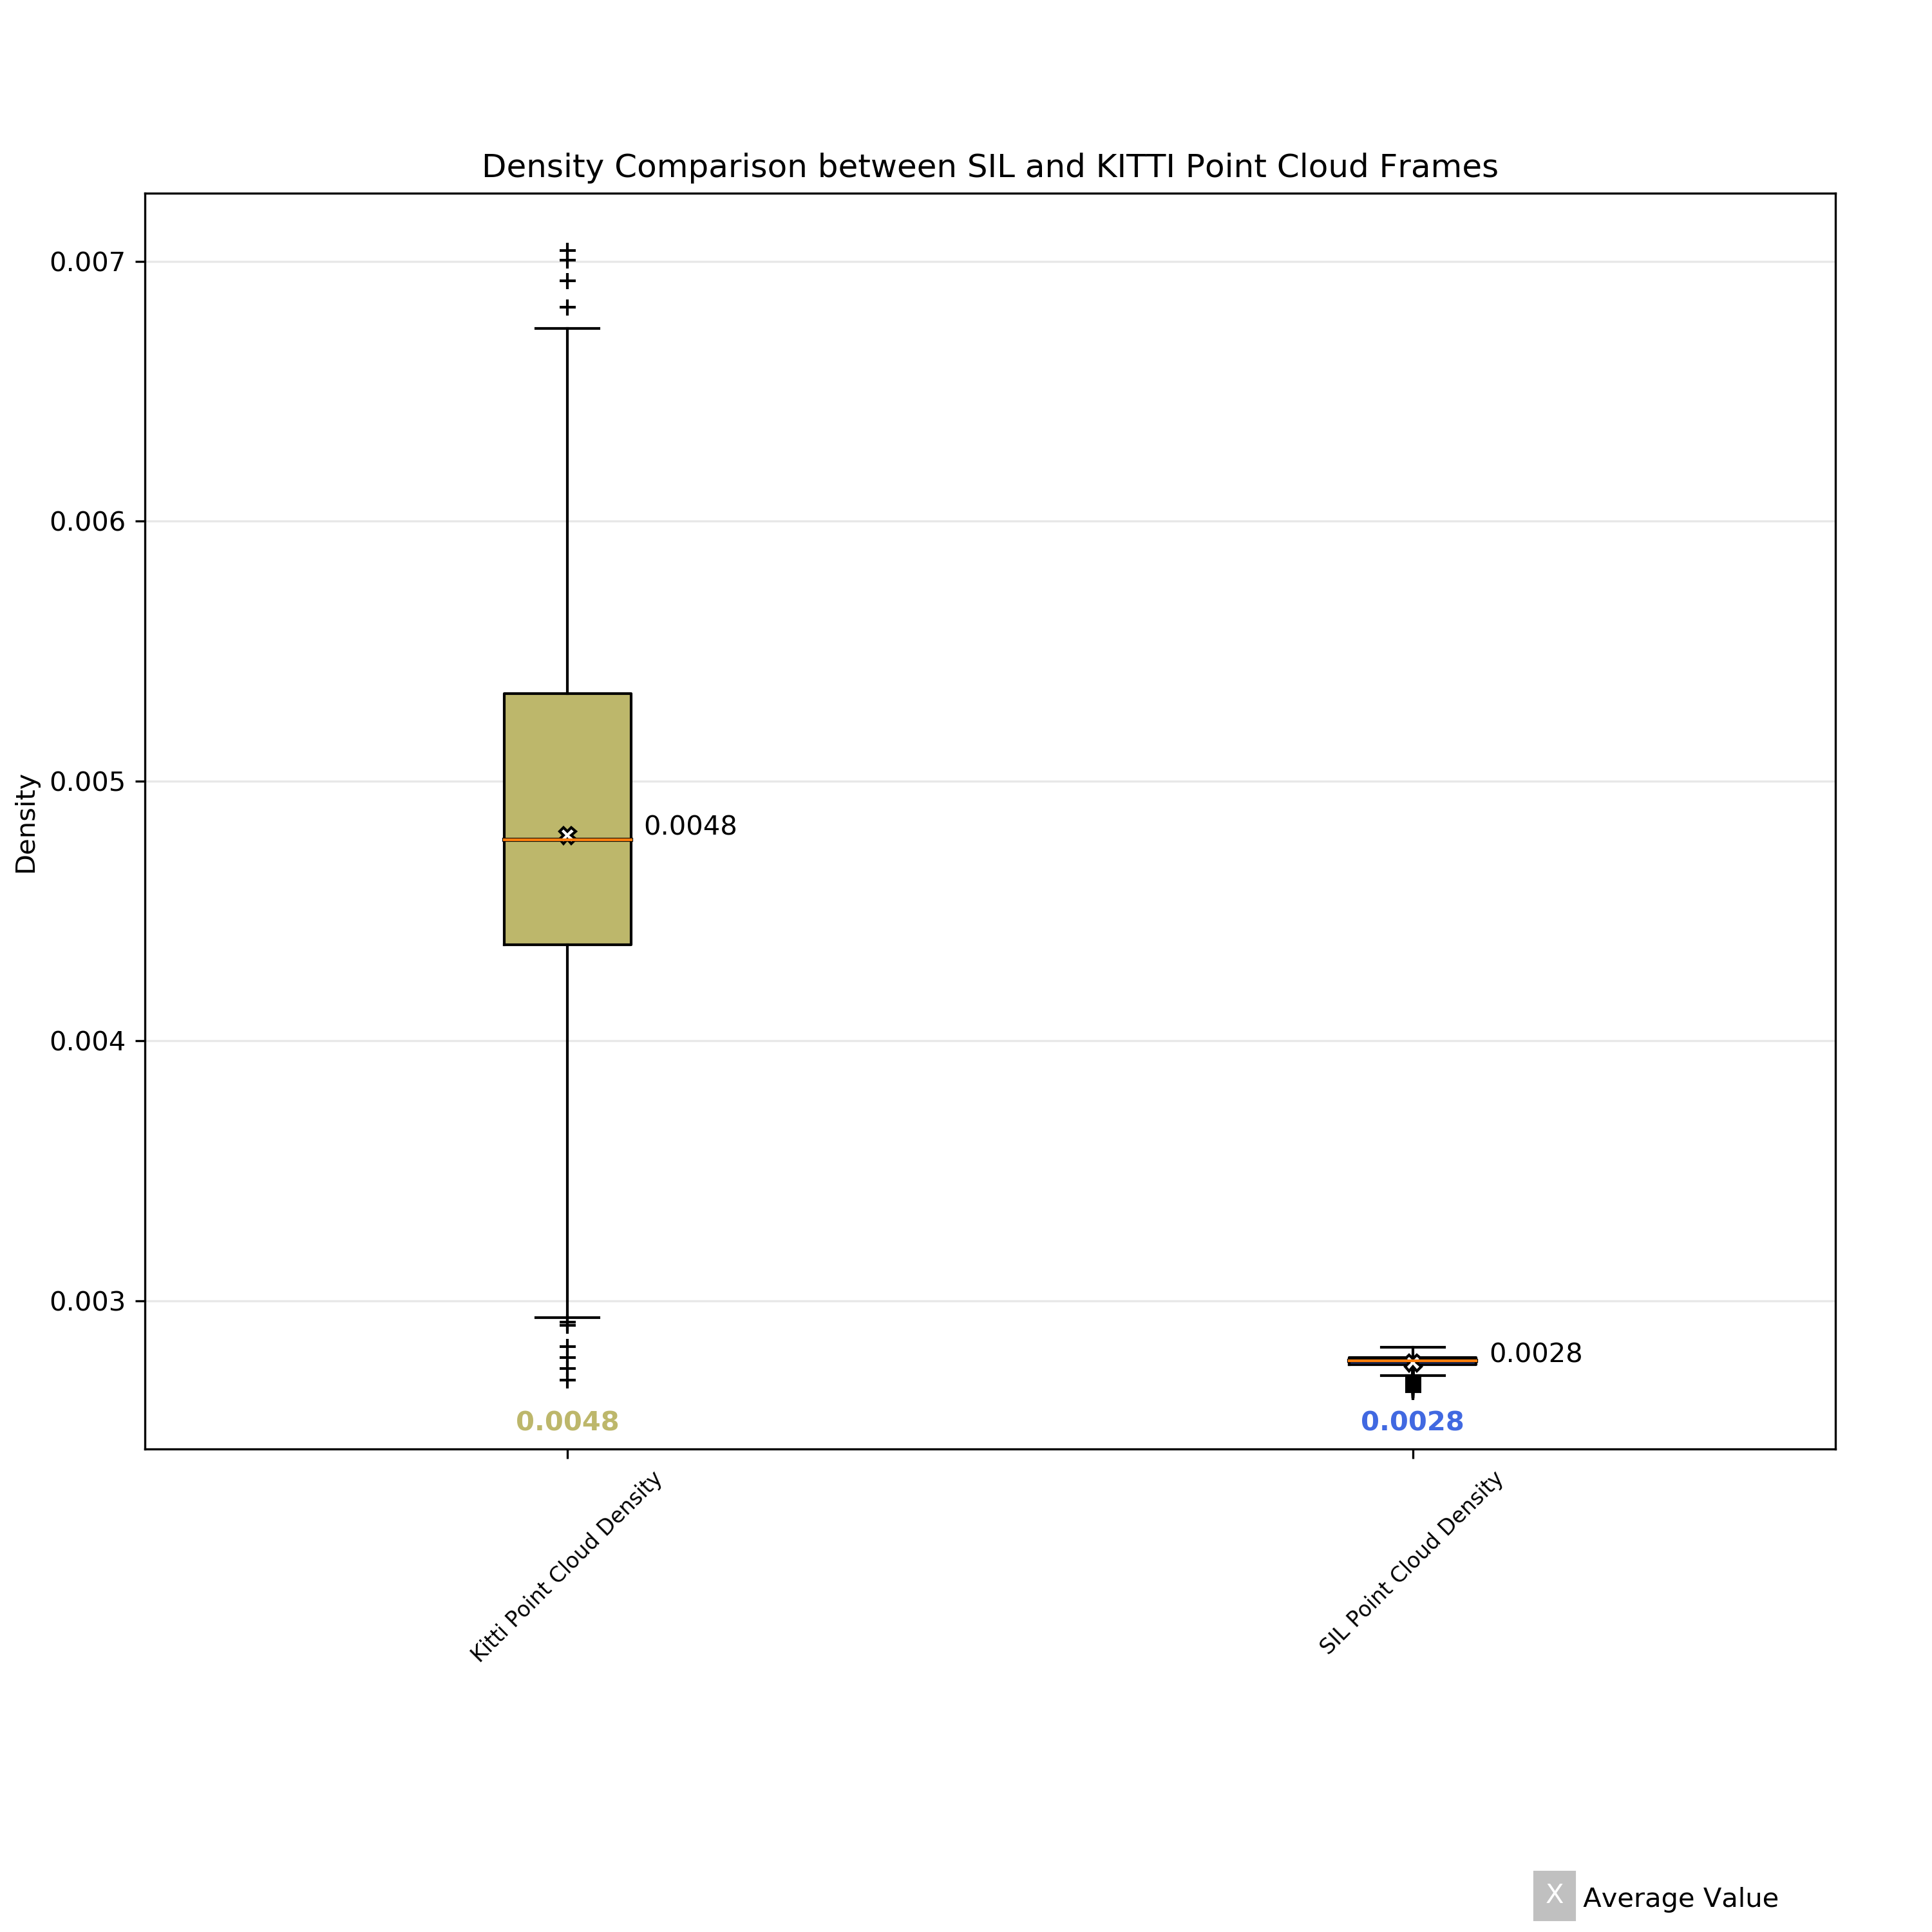
\includegraphics[width=0.6\linewidth]{images/density}
	\caption{Point Cloud Density}
	\label{fig:density}
\end{figure}


Following this evaluation, I established that there was a positive correlation between the performance of the LiDAR only models and the point cloud density of the input. As mentioned in the precious section, point clouds are sparse and as a result suffer from poor contour retrieval for objects. An increase in the point density could help alleviate this by allowing for more shape information to be recovered.


\section{Discussion}

